%\documentclass[12pt, openright,oneside, a4paper, english, brazil]{abntex2}
\documentclass[12pt,
               openright,
               oneside,
               a4paper,
							 section=TITLE,     % COMO SÃO AS LETRAS MAIÚSCULAS EM SEÇÃO
               subsection=Title,  % EM DIANTE ESCRITO NORMALMENTE
               english,brazil]{article}

\usepackage[a4paper,left=2.5cm,right=2.5cm,top=2.5cm,bottom=2.5cm]{geometry}

% ----------------------------
% Pacotes básicos 
% ----------------------------
% Referências
\usepackage[brazilian,hyperpageref]{}	
\usepackage{hyperref}
\usepackage[alf]{abntex2cite}			

% Fonte e codificação (acentuação)
%\usepackage{lmodern}       
%\renewcommand{\sfdefault}{ppl}
%\usepackage[T1]{fontenc}	
\usepackage{times}
\usepackage[T1]{fontenc}
\renewcommand*\familydefault{\sfdefault}
% Tabelas e Figuras
\usepackage{ctable}             
\usepackage{multirow}
\usepackage{array}
\usepackage{float}              
\usepackage{longtable}          
\usepackage{xcolor,colortbl}    
\usepackage{booktabs}           
\usepackage{graphicx}			
\usepackage{caption}  
\usepackage{subcaption}
\usepackage{epstopdf}    
\usepackage{rotating}

% Equações e símbolos
\usepackage{amsmath}            
\usepackage{nomencl} 
\usepackage{cleveref} 
\usepackage{calrsfs}
\usepackage{amssymb}
\usepackage{psfrag}
\usepackage[brazil]{babel}
% Texto
%\usepackage[showframe,heightrounded]{geometry}
\usepackage{geometry}
\usepackage{indentfirst}		
\usepackage{color}				
\usepackage{microtype} 			
\usepackage{lastpage}			
\usepackage{enumitem}                % Para os itens em letras
\usepackage{lipsum}
\usepackage{lastpage}
\usepackage{tablefootnote}
\usepackage{pdflscape}
\usepackage{scalefnt}
\usepackage[stable]{footmisc}
\usepackage{ragged2e}
% ----------------------------------------------------------
% Configurações do texto
% ----------------------------------------------------------

% Recuo do parágrafo :
\setlength{\parindent}{1.5cm}
\setlength{\parskip}{0cm} 
\geometry{a4paper}%,left=3cm,right=2cm,top=3cm,bottom=2cm} % SEMPRE BOM VER A DOCUMENTAÇÃO
\hoffset = -1in
\voffset = -1in
\oddsidemargin = 1.5cm
\topmargin = 2cm
\headheight = 0pt
\headsep = 6pt % multiplicar por 0.03515 para obter cm
\textheight = 249mm
\textwidth = 18cm
\marginparsep = 0pt
\marginparwidth = 0pt
\footskip = 6mm
%
%
%
\usepackage{array}
\newcolumntype{L}[1]{>{\raggedright\let\newline\\\arraybackslash\hspace{0pt}}m{#1}}
\newcolumntype{C}[1]{>{\centering\let\newline\\\arraybackslash\hspace{0pt}}m{#1}}
\newcolumntype{R}[1]{>{\raggedleft\let\newline\\\arraybackslash\hspace{0pt}}m{#1}}
%
%
%
\newtheorem{teorema}{Teorema}[section]
\newtheorem{propriedade}[teorema]{Condição}
\newtheorem{lema}[teorema]{Lema}
\newtheorem{corolario}[teorema]{Corolário}
\newtheorem{proposicao}[teorema]{Proposição}
\newtheorem{definicao}[teorema]{Definição}
\newtheorem{exemplo}[teorema]{Exemplo}
\newtheorem{af}[teorema]{AF}
\newtheorem{exercicio}[teorema]{Exercício}
\newtheorem{algoritmo}{Algoritmo}[section]
\newtheorem{exc}{}[section]
\newtheorem{impl}{}[section]
\newtheorem{hip}{H\hspace{-.12cm}}
\newtheorem{res}{R\hspace{-.12cm}}
%
%
%
\newcommand{\rel}{\Bbb R^{\ell}}
\newcommand{\rell}{\mathbb R^{\ell}_{+}}
\newcommand{\rr}{\mathbb R}
\newcommand{\bb}[1]{\boldsymbol{#1}}
\newcommand{\ol}[1]{\overline{#1}}
\newcommand{\hess}{\nabla^2(f(\bb{x}))}

\newcommand{\kktmax}[3]{
\begin{aligned}
& \underset{#1}{\text{maximizar}}
& & {#2} \\
& \text{sujeito a} 
& & {#3} \\
\end{aligned}}

\newcommand{\kktmin}[3]{
\begin{aligned}
& \underset{#1}{\text{minimizar}}
& & {#2} \\
& \text{sujeito a} 
& & {#3} \\
\end{aligned}}

%  Novos macros
\newcommand{\R}{\mathbb{R}}
\newcommand{\N}{\mathbb{N}}
\newcommand{\Rn}{{\R}^n}
\newcommand{\sumin}{\sum_{i=1}^n}
\newcommand{\Rl}{{\R}^\ell}
\newcommand{\Rm}{{\R}^m}
\newcommand{\ind}{1,\ldots,n}
%
%
%
%
%


\title{RIGIDEZ AMBIENTAL E COMÉRCIO INTERNACIONAL: O QUE EVIDENCIAM OS DADOS?}

\author{Pedro Milreu Cunha\thanks{Mestrando em economia aplicada no Programa de Pós-Graduação em Economia, Universidade Federal da Paraíba (UFPB). Email: <pedro.milreu@academico.ufpb.br>.} \and Rafael de Sousa Araújo\thanks{Doutorando em economia no Programa de Pós-Graduação em Economia, Universidade Federal de Pernambuco (UFPE). Email: <rafaelaraujo05@hotmail.com>.} \and Viviani Silva Lírio\thanks{Professora Titular do Departamento de Economia Rural da Universidade Federal de Viçosa (UFV). E-mail: <vslirio@ufv.br>.}}

\date{}
%
%
%
%
%
%
%
%
%


\begin{document}
\topmargin = 0.2cm
\maketitle

\setlength{\parindent}{0cm}

\textbf{RESUMO:} O objetivo do presente trabalho foi verificar a veracidade da hipótese de que a regulamentação ambiental de uma nação – capturada por meio de um score baseado no consumo energético do país – impacta em seus fluxos bilaterais de comércio internacional. Para tanto foram estimadas nove equações baseadas no modelo de gravidade, por meio de um painel contendo observações para 120 países durante o período de 2010-2014, utilizando o \textit{Poisson Pseudo-Maximum Likelihood Estimator (PPML)}. Os resultados apontam que, de forma geral, há um efeito significativo da \textit{proxy} utilizada para capturar a rigidez da legislação ambiental sobre os níveis de comércio internacional dos países da amostra.


\textbf{Palavras-chave}:  Modelo de gravidade. Comércio internacional. Meio ambiente.

\textbf{JEL:} F14. F18. Q56. 

\vspace{0.6cm}

\textbf{ABSTRACT:} The objective of the present work was to verify whether the hypothesis that a country’s environmental regulation – captured using a score based on the country’s energy consumption – affects their trade flows. In order to accomplish that, nine equations were estimated based on the gravity model, using a panel that includes data for 120 countries from 2010-2014. The estimation method was the Poisson Pseudo-Maximum Likelihood Estimator (PPML). The results show that, in general, there is a significant impact of the proxy used to capture the role of environmental legislation in the levels of international trade for the countries present in the sample.

\textbf{Keywords}: Gravity model. International trade. Environment.

\textbf{JEL:} F14. F18. Q56. 


\topmargin = 2cm
\setlength{\parindent}{1.5cm}

\maketitle

\section{\textbf{INTRODUÇÃO}}

Embora só se possa falar efetivamente em comércio internacional após o aparecimento dos estados nações, em virtude da adequação no uso dessa terminologia, o comércio entre regiões distantes ou entre populações diferentes data de muito antes das civilizações modernas. Há relatos que atestam para a existência de uma colônia mercantil assíria em Kanesh, Capadócia, ainda no século XIX a.C. \cite{Stearns2001}, bem como merece destaque a Rota da Seda, que foi amplamente utilizada entre os séculos II a.C. e XVIII, sendo central para a interação entre as regiões ocidental e oriental do mundo. \cite{Elisseeff2000}.\footnote{Informações mais detalhadas podem ser obtidas em \cite{Junguito2016, Vanham2019}}.

No entanto, foi a partir dos avanços tecnológicos obtidos na primeira Revolução Industrial - e com os subsequentes processos de inovação dela decorrentes -, que o comércio internacional passou a ter um papel mais determinante na economia mundial. Com a redução dos custos de transporte e com os incrementos na comunicação e na logística, as relações de troca internacionais tiveram sua realização facilitada, facultando a ampliação dos fluxos comerciais e a integração entre países. 

A constatação desse fenômeno pode ser feita, por exemplo, através da observação da relevância do comércio internacional ao longo do tempo, por meio do índice de abertura comercial dos países. Conforme pode-se verificar a partir dos dados apresentados na Figura \ref{fig:1}, durante praticamente todo o período analisado pelos autores – que perfizeram mais de 500 anos de história - houve aumento no índice, ocorrendo sua retração apenas em subperíodos específicos como guerras e grandes crises mundiais.

\begin{figure}[H]
	\centering
		\caption{Índice de abertura da economia mundial - 1500 a 2017 }
		{\subcaption*{(LS: Limite superior, LI: Limite inferior)}}%
        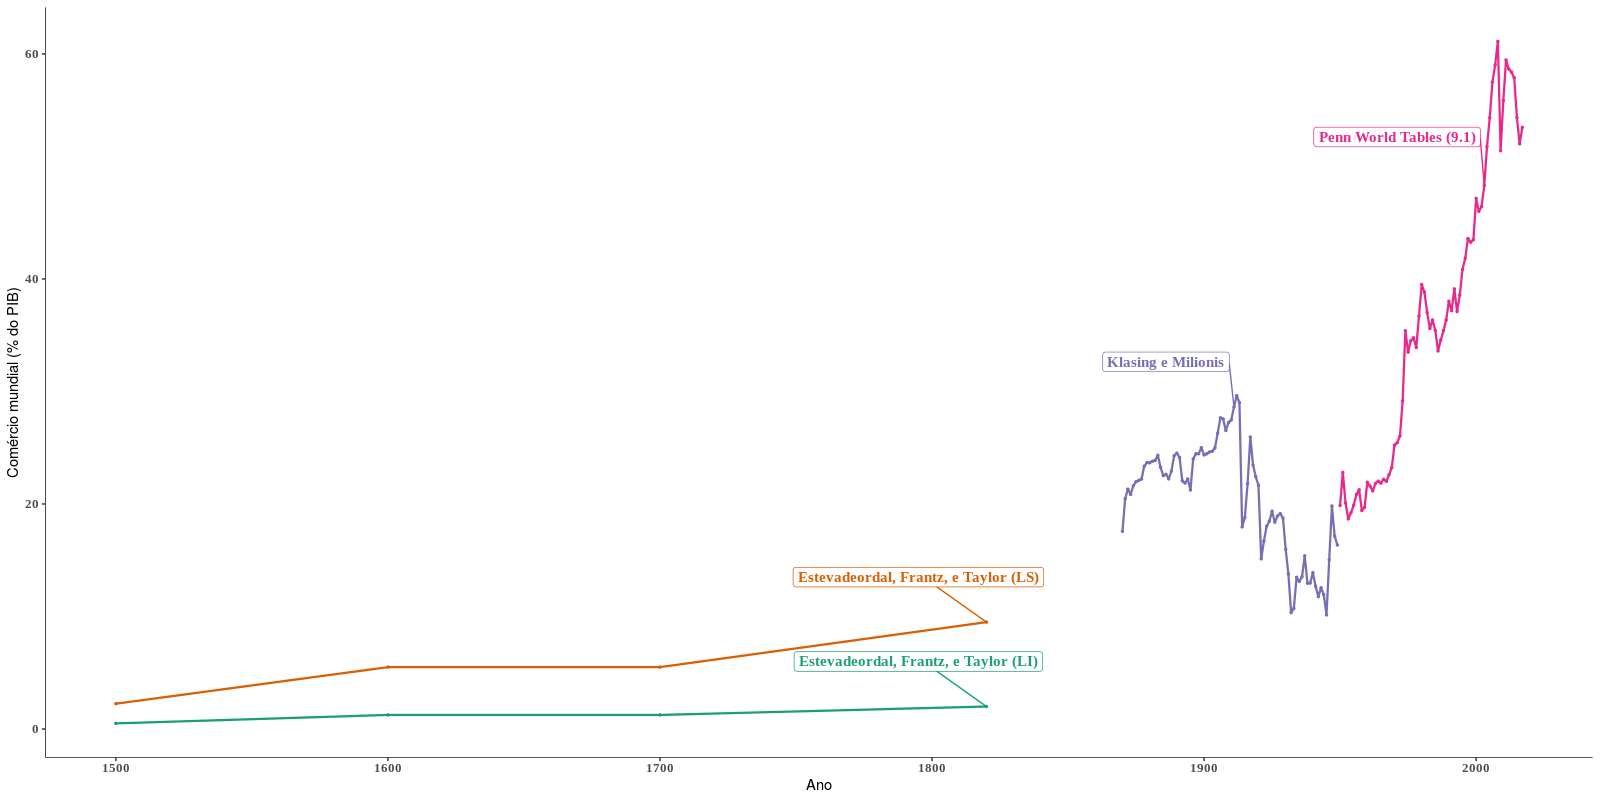
\includegraphics[width=\linewidth]{Figuras/globalizacao.png}
	\label{fig:1}
	\caption*{\RaggedRight  Fonte: \cite{Estevadeordal2003, Feenstra2015, Klasing2014}.}
\end{figure}

Em particular, após o final da revolução industrial foi quando se observou o primeiro incremento exponencial no índice de abertura da economia mundial. Além disso, na segunda metade do século XX, com a revolução da informação e o desenvolvimento de novas tecnologias, novamente verificou-se um aumento significativo no índice, chegando a atingir $61,11\%$ em 2008, tendo se mantido em média em $56,25\%$ desde então. 

Confirmando a importância do comércio internacional, \citeonline{Frankel1999} e \citeonline{Alcala2004} encontraram evidências de que a troca comercial é um dos fatores que impulsionam o crescimento econômico, sendo capaz de proporcionar aumento da competitividade das firmas, das economias de escala e da inovação. 

Apesar disso, é preciso cautela. Não obstante de uma forma agregada o efeito líquido do comércio internacional ser (geralmente) positivo, sobretudo em análises agregadas, há também consequências potencialmente negativas ou, ao menos, desafiadoras para muitos países. Nesse sentido, destaque-se a possibilidade de redução no nível de emprego \cite{Tuhin2015}, impactos na saúde \cite{Smith2015} e aumento da desigualdade regional \cite{Daumal2010, Pavcnik2017}. Em particular, há uma preocupação atual sobre como a abertura comercial pode estar afetando o meio-ambiente \cite{Frankel2008, Williams1993}.

Ainda não há um consenso na literatura acerca desta relação. \citeonline{Reynolds1991} aponta que embora o aumento na escala de produção possa significar mais poluição, desmatamento e outros danos ambientais, mudanças nos processos produtivos devido a inovação podem contornar esses problemas, equilibrando os impactos gerados com os benefícios do incremento produtivo. Para além disso, com o aumento da renda real dos indivíduos, há também a possibilidade de um aumento da demanda por qualidade ambiental (a chamada Curva de Kuznets ambiental\footnote{Referências complementares sobre este tema podem ser encontrados em \cite{Stern2004, Carvalho2010, Carvalho2013}}. 

\citeonline{Goncalves1998}, por seu turno, argumenta que a situação dos países em desenvolvimento é particularmente difícil, pois a vantagem comparativa desses países é largamente assentada na dotação de recursos naturais e em sua exploração; ademais, geralmente não dispõem de tecnologias de produção limpas ou encontram custos proibitivos em sua utilização (devido à condições históricas), de modo que a participação deles no comércio internacional têm um alto custo ambiental, como por exemplo as grandes plantações de soja no Brasil voltadas para exportação.

Tão importante quanto os estudos citados acima é a análise do impacto da regulamentação ambiental sobre os níveis de comércio, sendo esse o objeto de estudo do presente trabalho. Uma vez que teoricamente custos de controle ambiental podem desencorajar a produção de certos produtos, é plausível que países com normas mais flexíveis tenham uma vantagem de custos quando comparados àqueles com legislações ambientais mais estritas. \cite{Pethig1976, Siebert1977, McGuire1982}.

\citeonline{Tobey1990}, um dos primeiros a estudar empiricamente o tema, ao contrário do que aponta a teoria, não encontrou evidências que sustentem a hipótese de que uma legislação ambiental mais rígida causa uma alteração nos padrões de troca internacional das indústrias “sujas”, definidas pelo autor como aquelas cuja razão entre os custos com abatimento de poluição e os custos totais é maior do que 0.0185, como por exemplo as indústrias químicas e de mineração\footnote{O valor de corte de 0,0185 foi escolhido porque resulta em um conjunto de firmas que são geralmente consideradas como as mais poluidoras ao redor do mundo \cite{Tobey1990}}. 

\citeonline{VanBeers1997}, em trabalho semelhante ao desenvolvido por \citeonline{Tobey1990}, analisaram o impacto de regulamentações ambientais nos fluxos de comércio internacional, utilizando para isso uma análise empírica de vários países. Seus resultados apontaram que regulamentações mais estritas tem um forte impacto negativo nas exportações de commodities “sujas” de firmas “\textit{footloose}\footnote{São firmas que não dependem de um insumo de produção geograficamente específico.}”  ou “non-resource based” e nas importações de um modo geral. 

Um entrave à essas análises é a dificuldade em se obter uma medida para o rigor das legislações ambientais. Assim, os autores têm buscado utilizar proxies para essa variável, como por exemplo o score baseado no consumo de energia dos países utilizado por \citeonline{VanBeers1997} e no presente trabalho\footnote{É importante que pesquisas futuras busquem inovar de modo a criar uma medida mais fiel para a rigidez da legislação ambiental.} .

De fato, a preocupação ambiental cresceu muito nas últimas décadas, conforme evidencia-se pelas inúmeras conferências ambientais realizadas, como por exemplo a Conferência de Estocolmo (1972) e a Rio-92 (1992) – da qual resultaram sete importantes documentos oficiais\footnote{A Carta da Terra; A Convenção sobre Diversidade Biológica; A Convenção das Nações Unidas de Combate à Desertificação; A Convenção-Quadro das Nações Unidas sobre a Mudança do Clima; A Declaração dos princípios sobre Florestas; A Declaração do Rio sobre Meio Ambiente e Desenvolvimento e a Agenda 21} . Houve, ainda, a criação do Protocolo de Kyoto em 1997. Esse protocolo previa obrigações como reforma dos setores de energia e transportes; adoção de fontes energéticas renováveis, proteção das florestas dentre outras.

Em anos mais recentes foram realizadas outras conferências e ratificados outros acordos, como por exemplo a Cúpula do Desenvolvimento Sustentável (2015) e o Acordo de Paris (2015), respectivamente. Assim, tendo em vista a importância da temática atualmente, não se pode garantir que os resultados estimados com dados antigos continuem válidos, sendo necessárias novas análises.

Outra lacuna encontrada na literatura é a ausência de análises envolvendo países em desenvolvimento. \citeonline{Tobey1990} e \citeonline{VanBeers1997}, por exemplo, tratam de países membros da Organização para a Cooperação e Desenvolvimento Econômico (OCDE). Os autores apontam a dificuldade de obtenção de dados para os países em desenvolvimento e sua heterogeneidade como razões para sua exclusão da análise.

Nesse sentido, tendo por base a hipótese de que o cenário ambiental de um país tem efeito sobre seus fluxos de comércio internacional, o presente trabalho tem por objetivo analisar a adequação dessa hipótese para as relações comerciais de um conjunto de cento e vinte países entre os anos de 2010-2014. Espera-se, com isso, contribuir com o avanço do entendimento sobre a interação entre os dois temas e com a literatura nacional sobre o assunto.

\section{Modelo de gravidade}
 Proposto inicialmente por \citeonline{Tinbergen1962} \footnote{\citeonline{Isard1954} é o autor do trabalho original sobre o modelo de gravidade. \citeonline{Tinbergen1962} foi quem primeiro aplicou o modelo às trocas internacionais.} , o modelo postula que, assim como a lei de gravitação universal da física, as relações de troca entre países são inversamente proporcionais à distância entre eles (distância entre os corpos) e diretamente proporcionais ao tamanho das economias deles (massa dos corpos). Matematicamente, essa relação pode ser expressa como em (\ref{eq:1}):
 
 \begin{equation} \label{eq:1} F_{ij} = G \cdot \frac{M_i \cdot M_j}{D_{ij}} \end{equation}
 
onde:

 $F_{ij}$: fluxo comercial entre os países $i$ e $j$;
 
 $G$: é uma constante;
 
 $M_i$ e $M_j$: dimensão da economia do país $i$ e $j$, respectivamente;
 
 $D_{ij}$: distância entre os países $i$ e $j$.

Apesar dos esforços iniciais, é importante destacar que as estimações do modelo de gravidade aplicadas ao comércio internacional realizadas nas décadas de 1960 e 1970 careciam de maior fundamentação teórica, fazendo com que esta caísse em desuso durante algum tempo \cite{Baldwin2006}. O desenvolvimento do trabalho de \citeonline{Anderson1979}, no qual foram apresentados microfundamentos para o modelo, permitiu o retorno e a extensão de suas aplicações. 

Nesta proposta, o autor, fazendo uso das funções de despesa, diferenciação por origem e preferências do tipo \textit{Constant Elasticity of Substitution (CES)}, derivou uma equação gravitacional teórica. Outros trabalhos que buscam alicerçar o modelo gravitacional na teoria econômica são \cite{Bergstrand1985, Bergstrand1989, Deardorff1998}.

\citeonline{Anderson2003} avançaram o arcabouço teórico do modelo de gravidade ao analisarem os resultados obtidos por \citeonline{McCallum1995}\footnote{\citeonline{McCallum1995} deu origem ao “border puzzle” devido ao resultado encontrado em seu trabalho, apontando que a fronteira entre o Canadá e os Estados Unidos gerou trocas entre as províncias canadenses que são 22 vezes maiores que as trocas entre as províncias canadenses e os estados norte americanos para o ano de 1998.}  e apresentarem os conceitos de resistência bilateral e resistência multilateral. Segundo os autores, para além dos fatores de resistência à troca entre cada par de países (resistência bilateral), há de se levar em conta também os fatores de resistência de cada país com todos os demais (resistência multilateral). Uma vez corrigida essa omissão, foram encontrados os resultados esperados.
 
Com o passar dos anos, o modelo foi sendo aprimorado, de forma a incorporar mais variáveis, tornando possível diversas análises. \citeonline{Egger2011, DeSousa2012, Cipollina2010} são exemplos de trabalhos que fazem uso do modelo de gravidade para analisar os impactos de acordos comerciais regionais e de acordos de troca preferenciais. 

\citeonline{VanBeers1997} e \citeonline{Tobey1990}, por outro lado, utilizaram o modelo aumentado em sua análise sobre o efeito de uma legislação ambiental mais estrita sobre o comércio internacional. Por fim, a análise proposta no presente trabalho também será realizada mediante uso do modelo de gravidade, de modo semelhante aos autores citados acima.\footnote{O modelo de gravidade é o carro-chefe das análises de comércio internacional. Assim, foram citados aqui apenas aqueles artigos considerados mais relevantes para o objeto de estudo.}. 

\section{METODOLOGIA}

Nesta seção serão apresentados os dados, com suas respectivas fontes e estatísticas descritivas e os mecanismos utilizados para alcançar os objetivos propostos no estudo. Para isso, a seção será dividida em cinco partes, sendo elas respectivamente, i) fonte de dados; ii) a forma de construção do score de rigidez ambiental; iii) estatísticas descritivas; iv) o modelo estimado e v) o método utilizado para a sua estimação e suas limitações.

\subsection{Fontes de dados}

Os dados relacionados aos fluxos de comércio bilaterais  foram obtidos junto à \textit{United Nations Commodity Trade Statistics Database (COMTRADE)}. Os referentes à existência de fronteira, língua comum e às distâncias entre os países foram coletados junto ao \textit{Centre D’Estudes Prospectives et d’Informations Internationales (CEPII)}. Por fim, os dados sobre o Produto Interno Bruto (PIB) e a intensidade do uso de energia e sua variação foram obtidos utilizando o banco de dados do \textit{World Bank} (os \textit{scores} de rigidez ambiental são de construção própria do autor)\footnote{Os fluxos de comércio bilaterais e o PIB são medidos em dólares correntes; a distância é medida em quilômetros e o consumo de energia é medido em quilograma equivalente de óleo de uso de energia por \$1.000 de Produto Interno Bruto (PIB) (paridade de poder de compra constante de 2011).}.

Essas informações foram coletadas para uma amostra de 120 países, durante um período de 5 anos. A escolha dos países visou a obtenção de um grupo relativamente grande e heterogêneo, obtendo-se uma amostra diversificada, composta não apenas por países desenvolvidos, permitindo assim uma análise mais robusta da problemática em questão. A escolha do espaço temporal foi definida em função da disponibilidade de dados. Com isso, foram obtidas 71400 observações. 

\subsection{A construção do \textit{score} de rigidez da legislação ambiental}

Uma boa proxy para a rigidez da legislação ambiental deve ser orientada pelo resultado\footnote{Do inglês “output-oriented”.}  das medidas legislativas, não devendo considerar apenas os gastos com abatimento e controle de poluição\footnote{A construção desse score é baseada nos trabalhos de \cite{VanBeers1997, Tobey1990}}. Isso se deve ao fato de que um indicador assim construído captará também os impactos de medidas como subsídios e outros tipos de assistência financeira que possam distorcer os resultados das políticas ambientais. Além disso, para os autores, o indicador deve se ater ao máximo ao “\textit{polluter pays principle}”\footnote{Princípio diz que quem for responsável pela poluição também deve ser responsável pelo pagamento dos custos causados por ela.} . Seguindo esta orientação, foram então utilizadas as seguintes variáveis para a construção do indicador:

i) Mudança de intensidade de energia de cada país durante o período observado;

ii) Nível de intensidade de energia anual de cada país durante o período observado medido em quilograma equivalente de óleo por \$1.000 PIB (paridade de poder de compra constante de 2011).

A ideia por trás dessa escolha é que países com alta intensidade de uso de energia, e que conseguiram reduzir esse valor ao longo do período analisado, o fizeram devido à uma legislação ambiental mais estrita. Para a criação do \textit{score} foram realizadas as seguintes etapas:

i) Os valores das variáveis foram ordenados em ordem decrescente, atribuindo 1 para o país com o pior resultado (valor mais baixo), 2 para o segundo pior e assim por diante, até atribuir o valor 120 para o país com o melhor resultado (valor mais alto);

ii) Para 2010 o \textit{score} de cada país foi obtido dividindo o valor obtido para o nível de intensidade de energia no passo anterior por 120 (número de países na amostra); 

iii) Para os demais anos, primeiro somou-se os valores obtidos para a mudança de intensidade e de nível de intensidade de energia. Essa nova quantidade foi novamente classificada em ordem decrescente e, por fim, esse último valor foi dividido por 120, gerando o \textit{score} final de cada país para os anos de 2011-2014.

\subsection{Estatísticas descritivas}

Em primeiro lugar tem-se a Tabela \ref{tab:descritivas_total}, que mostra as estatísticas descritivas considerando todos os países da amostra. Pode-se observar que há grande variabilidade nos valores dos fluxos bilaterais, independentemente do tipo que sejam. Além disso, os países apresentam uma distância média em logaritmo de $8,617$ km. No tocante às variáveis \textit{dummy}, têm-se que $2,4\%$ dos países fazem fronteira e $10\%$ têm uma língua em comum. Em relação ao PIB, tem-se que o valor médio em logaritmo é de $25,418$, com uma amplitude relativamente alta. Por fim, o \textit{score} médio obtido pelos membros da amostra é de $0,502$.

\begin{table}[H] 
	\centering 
	\caption{Estatísticas descritivas - amostra completa} 
	\label{tab:descritivas_total} 
	\begin{tabular}{@{\extracolsep{5pt}}lccccc} 
		\\[-1.8ex]\toprule 
		Estatística & \multicolumn{1}{c}{N} & \multicolumn{1}{c}{Média} & \multicolumn{1}{c}{Desv. pad.} & \multicolumn{1}{c}{Mín.} &  \multicolumn{1}{c}{Máx.} \\ 
		\midrule \\[-1.8ex] 
		Fluxo total & 71400 & 1025669 & 7933239 & 0 & 397099250 \\ 
		Fluxo NRB & 71400 & 58745398 & 463351629 & 0 &  22058296512 \\ 
		Fluxo RB & 71400 & 172312629 & 1281481999 & 0 &  68233426147 \\ 
		Fronteira & 71400 & 0,024 & 0,152 & 0 & 1 \\ 
		Língua comum & 71400 & 0,100 & 0,299 & 0 & 1 \\ 
		$\ln$(Distância) & 71400 & 8,617 & 0,836 & 4,662 & 9,886 \\ 
		Score exportação & 71400 & 0,502 & 0,289 & 0,008 &  1 \\ 
		Score importação & 71400 & 0,502 & 0,289 & 0,008 &  1,000 \\
		$\ln$(PIB) & 71400 & 25,418 & 1,799 & 21,995 & 30,494 \\ \bottomrule \\[-1.8ex] 
	\end{tabular}
\caption*{\RaggedRight  Fonte: elaboração própria baseada nos dados disponíveis em \cite{Cepii2019, Comtrade2019, WorldBank2019}.}
\end{table} 
Considerando agora apenas os $50\%$ mais ricos, cujos dados encontram-se dispostos na Tabela \ref{tab:descritivas_ricos}, têm-se um pequeno na proporção de países que fazem fronteira, aumentando para $3,9\%$. A existência de um idioma comum, por outro lado, tem seu percentual reduzido para $9,7\%$, assim como a distância média, que diminui para $8,589$, e o \textit{score} médio dos países observados que cai para $0,491$. 

\begin{table}[H] \centering 
	\caption{Estatísticas descritivas - amostra dos 50\% mais ricos} 
	\label{tab:descritivas_ricos} 
	\begin{tabular}{@{\extracolsep{5pt}}lccccc} 
		\\[-1.8ex]\toprule 
		Estatística & \multicolumn{1}{c}{N} & \multicolumn{1}{c}{Média} & \multicolumn{1}{c}{Desv. pad.} & \multicolumn{1}{c}{Mín.} &  \multicolumn{1}{c}{Máx.} \\ 
		\midrule \\[-1.8ex] 
		Fluxo total & 17700 & 3814278 & 15578088 & 0 &  397099250 \\ 
		Fluxo NRB & 17700 & 218542021 & 909871558 & 0 & 22058296512 \\ 
		Fluxo RB & 17700 & 285211733 & 1756222185 & 0 &  68233426147 \\ 
		Fronteira & 17700 & 0,039 & 0,194 & 0 & 1 \\ 
		Língua comum & 17700 & 0,097 & 0,296 & 0 & 1 \\ 
		$\ln$(Distância) & 17700 & 8,589 & 0,896 & 4,952 & 9,886 \\ 
		Score exportação & 17700 & 0,491 & 0,278 & 0,008 &  1 \\ 
		Score importação & 17700 & 0,491 & 0,278 & 0,008 &  1 \\ $\ln$(PIB) & 17700 & 26,928 & 1,154 & 24,965 & 30,494\\
		\bottomrule \\[-1.8ex] 
	\end{tabular} 
\caption*{\RaggedRight  Fonte: elaboração própria baseada nos dados disponíveis em \cite{Cepii2019, Comtrade2019, WorldBank2019}.}
\end{table} 
Por fim, ao considerar apenas os $50\%$ mais pobres (Tabela \ref{tab:descritivas_pobres}), há uma redução na distância média entre os países, caindo para $8,605$ km, bem como uma diminuição na proporção de países que fazem fronteira, atingindo o patamar de $1,8\%$, e o PIB, apresentando um valor médio em logaritmo de $23,907$. A existência de uma língua comum, por outro lado, aumenta para o percentual de $10,2\%$ e o \textit{score} médio torna-se maior também, alcançando $0,512$.\footnote{Todas as comparações são considerando o caso base no qual todos os países estão presentes na amostra.}

\begin{table}[H] \centering 
	\caption{Estatísticas descritivas - amostra dos 50\% mais pobres} 
	\label{tab:descritivas_pobres} 
	\begin{tabular}{@{\extracolsep{5pt}}lccccc} 
		\\[-1.8ex]\toprule 
		Estatística & \multicolumn{1}{c}{N} & \multicolumn{1}{c}{Média} & \multicolumn{1}{c}{Desv. pad.} & \multicolumn{1}{c}{Mín.} &  \multicolumn{1}{c}{Máx.} \\ 
		\midrule \\[-1.8ex] 
		Fluxo total & 17700 & 16199,340 & 122154,100 & 0 & 4594009 \\ 
		Fluxo NRB & 17700 & 994299,300 & 7935722 & 0 & 178819323 \\ 
		Fluxo RB & 17700 & 56997647 & 537979402 & 0 & 22270580757 \\ 
		Fronteira & 17700 & 0,018 & 0,133 & 0 & 1 \\ 
		Língua comum & 17700 & 0,102 & 0,302 & 0 &  1 \\ 
		$\ln$(Distância) & 17700 & 8,605 & 0,819 & 4,903 & 9,843 \\ 
		Score exportação & 17700 & 0,512 & 0,299 & 0,008  & 1\\ 
		Score importação & 17700 & 0,512 & 0,299 & 0,008  & 1 \\ 
		$\ln$(PIB) & 17700 & 23,907 & 0,761 & 21,955 & 25,132\\
		\bottomrule \\[-1.8ex] 
	\end{tabular} 
\caption*{\RaggedRight  Fonte: elaboração própria baseada nos dados disponíveis em \cite{Cepii2019, Comtrade2019, WorldBank2019}.}
\end{table} 


\subsection{Especificação do modelo}

Uma das etapas relevantes do estudo consiste em definir, ou especificar, as equações a serem estimadas, uma vez que sua composição deve refletir a intenção da pesquisa e permitir as inferências pretendidas. As equações estimadas no presente trabalho têm a seguinte forma:

\begin{align} \label{eq:2}
 X_{ijt} = \exp & \{ \sum \gamma_j + \beta_0 \cdot contig_{ij} + \beta_1 \cdot comlang\_off_{ij}  \nonumber \\ & + \beta_2 \cdot \ln(distwces)_{ij} + \beta_3 \cdot SCO_{it} + \beta_4 \cdot SCO_{jt} \nonumber \\ & + \beta_5 \cdot \ln(PIB)_{it} + \beta_6 \cdot \ln(PIB)_{jt} \} \cdot \epsilon_{ijt}
\end{align}

onde:

$X_{ijt}$ representa os fluxos comerciais bilaterais entre os países $i$ (exportador) e $j$ (importador) para o ano $t$;  $\gamma_j$ representa os efeitos fixos do país importador; $contig_{ij}$ é uma variável dummy que assume valor 1 caso $i$ e $j$ façam fronteira e 0 caso contrário; $comlang\_off_{ij}$ é uma variável dummy que assume valor 1 caso $i$ e $j$ tenham um idioma comum; $\ln(distwces)_{ij}$ é o logaritmo da distância entre os países $i$ e $j$; $SCO_{it}$ e $SCO_{jt}$ representam respectivamente os scores de rigidez ambiental de $i$ e $j$ para o ano $t$; $\ln(PIB)_{it}$ e $\ln(PIB)_{jt}$ são, respectivamente, os logaritmos do PIB do país exportador e do país importador no ano $t$; e $\epsilon_{ijt}$ é o termo de erro com $E[\epsilon_{ijt} |K=1]$, onde $K$ é o vetor de variáveis explicativas do modelo.

Foram estimadas nove equações, divididas em três grupos principais, cuja única diferença é a variável dependente. Dentro de cada grupo foram estimadas equações para todos os países da amostra, para os 50\% mais ricos e para os 50\% mais pobres (baseado na média do PIB para o período analisado). Para o primeiro grupo, foram utilizados os fluxos bilaterais totais como variável explicada. Para o segundo, fez-se uso dos fluxos “sujos” de \textit{commodities} que são "\textit{resouce-based}" como variável dependente (as indústrias sujas são aquelas que gastam 1\% ou mais de sua receita de vendas com custos de controle e abatimento de poluição). Para o último, foram utilizadas apenas os fluxos “sujos” que eram “non-resource based”\footnote{As firmas classificadas como “sujas” e/ou “footloose” encontram-se no apêndice. Convém destacar que os setores apresentados são considerados sujos na “média”, ou seja, nada afirma-se sobre firmas específicas, podendo estas serem sujas ou não.} . 

Para os fluxos totais agregados, espera-se que a existência de fronteira ($\beta_0$) e um idioma comum ($\beta_1$), bem como os PIBs dos respectivos países ($\beta_5$ e $\beta_6$) se relacionem positivamente com os fluxos bilaterais, enquanto a distância deve afetá-los negativamente ($\beta_2$). Baseado em \citeonline{VanBeers1997}, há expectativa a priori de que os scores de rigidez da legislação ambiental têm relação negativa com o volume de trocas ($\beta_3$ e $\beta_4$).

Por outro lado, para os demais fluxos, em especial para as subamostras de países ricos e países pobres, não há expectativa a priori sobre o sinal de nenhuma das variáveis.

\subsection{Estratégia de estimação e seus condicionantes}

Visando controlar as resistências bilaterais e multilaterais, conforme \citeonline{Anderson2003} instrui, foram estimados efeitos fixos invariantes no tempo para cada importador.\footnote{Optou-se pelos efeitos fixos por importador e não por efeitos fixos por pares de países pois estão sendo utilizadas variáveis bilaterais para controle, além dos próprios scores. O uso de apenas efeitos fixos por exportador não teve resultados significativos.} Assim, características específicas de cada região puderam ser capturadas, evitando o viés da variável omitida. 

Além disso, para as variáveis contínuas, optou-se pela aplicação da transformação logarítmica, o que faz com que os coeficientes estimados para elas possam ser interpretados como simples elasticidades.

Tendo por base o trabalho de \citeonline{Silva2006}, referência na área, optou-se pela estimação utilizando o \textit{Poisson Pseudo-Maximum Likelihood Estimator (PPML)}, uma vez que esse estimador é robusto à heterocedasticidade causada pela forma funcional do modelo e, ao contrário do estimador de Mínimos Quadrados Ordinários (MQO), é apropriado para lidar com fluxo bilaterais nulos, tornando desnecessária a exclusão ou manipulação dessas observações. Além disso, com o PPML é possível trabalhar com o modelo em sua forma exponencial, não sendo necessário transformá-lo, evitando assim maiores problemas relacionados ao viés do estimador\footnote{Àqueles interessados no desenvolvimento e nas demonstrações técnicas acerca do PPML podem consultar \citeonline{Silva2006}, onde os autores demonstram como a transformação logarítmica da variável dependente pode tornar os resultados viciados, além de proporem uma solução alternativa robusta à heterocedasticidade e capaz de lidar com observações de valor zero na forma do estimador PPML.}.

Por fim, uma vez que os erros de países geograficamente próximos são provavelmente correlacionados, optou-se por \textit{clusterizar} os dados com base na variável $\ln(distwces)$, ou seja, a distância entre os países.


\section{RESULTADOS E DISCUSSÃO}

O objetivo do presente artigo era verificar qual a relação existente entre a rigidez ambiental de um país e seus fluxos bilaterais de comércio internacional. Para tanto, foram estimados nove modelos separados em três grupos. A discussão dos resultados obtidos é feita na sequência, sendo apresentadas duas tabelas para cada grupo: i) resultados da estimação; ii) interpretação dos resultados. 

Na Tabela \ref{tab:resultados_nrb} abaixo, são apresentados os resultados dos modelos que consideram apenas os fluxos "sujos"  e que são "\textit{non-resource-based}".
\begin{table}[H]
\centering
\caption{Estimativas - fluxos sujos e "non-resource based"}
\label{tab:resultados_nrb}
\begin{tabular}{lccc}
 & \multicolumn{3}{c}{Amostra} \\ \cmidrule(l){2-4} 
Variável & Agregado & 50\% mais ricos & 50\% mais pobres \\ \midrule
\multirow{2}{*}{constante} & -11,4543$^{***}$ & -10,3384$^{***}$ & 4,7640 \\
 & (1,3963) & (2,4282) & (6,0216) \\
\multirow{2}{*}{$\ln$(distância)} & -1,0927$^{***}$ & -1,0606$^{***}$ & -2,0787$^{***}$ \\
 & (0,0066) & (0,0112) & (0,0584) \\
\multirow{2}{*}{contiguidade} & 0,2814$^{***}$ & 0,2713$^{***}$ & -0,5000$^{***}$ \\
 & (0,0156) & (0,0263) & (0,1010) \\
\multirow{2}{*}{língua comum} & -0,0494$^{***}$ & -0,0725$^{***}$ & 0,5669$^{***}$ \\
 & (0,0157) & (0,0267) & (0,1051) \\
\multirow{2}{*}{score origem} & 0,4373$^{***}$ & 0,4204$^{***}$ & 0,4352$^{***}$ \\
 & (0,0197) & (0,0333) & (0,1107) \\
\multirow{2}{*}{score destino} & -0,0597$^{**}$ & -0,0650 & -0,1004 \\
 & (0,0281) & (0,0478) & (0,1480) \\
\multirow{2}{*}{$\ln$(PIB origem)} & 0,9766$^{***}$ & 0,9554$^{***}$ & 0,7666$^{***}$ \\
 & (0,0036) & (0,0068) & (0,0525) \\
\multirow{2}{*}{$\ln$(PIB destino)} & 0,4494$^{***}$ & 0,4200$^{***}$ & 0,1752 \\
 & (0,0545) & (0,0948) & (0,2591) \\ \midrule
Observações& 71400&17700&17700\\
\bottomrule\bottomrule
\multicolumn{4}{l}{\emph{Todos os modelos foram estimados com efeitos fixos por importador.}}\\
\multicolumn{4}{l}{\emph{Erros-padrão robustos clusterizados por distwces entre parênteses.}}\\
\multicolumn{4}{l}{\emph{Níveis de significância: ***: 0,01, **: 0,05, *: 0,1}}\\
\end{tabular}
\caption*{\RaggedRight  Fonte: elaboração própria baseada nos dados disponíveis em \cite{Cepii2019, Comtrade2019, WorldBank2019}.} 
\end{table}
Para todas as equações estimadas, a distância apresenta sinal negativo, com valores em torno de $-1,1$ para a amostra agregada e para os países mais ricos, e atingindo $-2,1$ aproximadamente para os mais pobres. De modo semelhante, países que fazem fronteira apresentam um maior volume de comércio, com exceção da amostra dos países mais pobres, caso no qual esse efeito é negativo. Além disso, enquanto uma língua comum diminui os fluxos bilaterais para os dois primeiros grupo, para o terceiro há um aumento. Por fim, o efeito positivo do tamanho das economias dos países é observado em quase todos os modelos, sendo o PIB do país importador para a amostra dos mais pobres a única variável não-significativa.

Na Tabela \ref{tab:interpretação_nrb}, são resumidas as interpretações dos resultados de cada amostra. O \textit{score} do país exportador se mostrou significativo em todas as amostras, se relacionando positivamente com a magnitude do comércio internacional. Isso indica que quanto maior a rigidez ambiental no país de origem, maior a quantidade de exportações. Para o \textit{score} do país importador, foi constatado um efeito negativo na amostra agregada e nenhum efeito nas demais. Uma possível explicação é que os governos podem estar fazendo uso de políticas ambientais como substitutos para barreiras comerciais.

\begin{landscape}
\begin{table}
\centering
\caption{Interpretação dos resultados - fluxos sujos e "non-resource based"}
\label{tab:interpretação_nrb}
\begin{tabular}{@{}lccc@{}}
 & \multicolumn{3}{c}{Amostra} \\ \cline{2-4} 
Variável & Agregado & 50\% mais ricos & 50\% mais pobre \\ \midrule
distância & \begin{tabular}[c]{@{}c@{}}Um aumento de $1\%$ na distância está\\ relacionado a uma redução de $1,09\%$\\ nos fluxos bilaterais de comércio\end{tabular} & \begin{tabular}[c]{@{}c@{}}Um aumento de $1\%$ na distância está\\ relacionado a uma redução de $1,06\%$\\ nos fluxos bilaterais de comércio\end{tabular} & \begin{tabular}[c]{@{}c@{}}Um aumento de $1\%$ na distância está\\ relacionado a uma redução de $2,08\%$\\ nos fluxos bilaterais de comércio\end{tabular} \\ \midrule
contiguidade & \begin{tabular}[c]{@{}c@{}}Fazer fronteira está relacionado a um\\ aumento de $28,14\%$ nos fluxos \\ bilaterais de comércio\end{tabular} & \begin{tabular}[c]{@{}c@{}}Fazer fronteira está relacionado a um\\ aumento de $27,13\%$ nos fluxos \\ bilaterais de comércio\end{tabular} & \begin{tabular}[c]{@{}c@{}}Fazer fronteira está relacionado a uma\\ redução de $39,35\%$ nos fluxos \\ bilaterais de comércio\end{tabular} \\ \midrule
língua comum & \begin{tabular}[c]{@{}c@{}}Ter uma linguagem comum está \\ relacionado a uma redução de $4,94\%$\\ nos fluxos bilaterais de comércio\end{tabular} & \begin{tabular}[c]{@{}c@{}}Ter uma linguagem comum está \\ relacionado a uma redução de $7,24\%$\\ nos fluxos bilaterais de comércio\end{tabular} & \begin{tabular}[c]{@{}c@{}}Ter uma linguagem comum está \\ relacionado a um aumento de $76,28\%$\\ nos fluxos bilaterais de comércio\end{tabular} \\ \midrule
score origem$^*$ & \begin{tabular}[c]{@{}c@{}}O score do país exportador se relaciona\\ positivamente com os fluxos bilaterais\\ de comércio\end{tabular} & \begin{tabular}[c]{@{}c@{}}O score do país exportador se relaciona\\ positivamente com os fluxos bilaterais\\ de comércio\end{tabular} & \begin{tabular}[c]{@{}c@{}}O score do país exportador se relaciona\\ positivamente com os fluxos bilaterais\\ de comércio\end{tabular} \\ \midrule
score destino$^*$ & \begin{tabular}[c]{@{}c@{}}O score do país importador se relaciona\\ negativamente com os fluxos bilaterais\\ de comércio\end{tabular} & Não foi significativa & Não foi significativa \\ \midrule
PIB origem & \begin{tabular}[c]{@{}c@{}}Um aumento de $1\%$ no PIB do país\\ exportador está relacionado a um \\ aumento de $0,98\%$ nos fluxos bilaterais\\ de comércio\end{tabular} & \begin{tabular}[c]{@{}c@{}}Um aumento de $1\%$ no PIB do país\\ exportador está relacionado a um \\ aumento de $0,95\%$ nos fluxos bilaterais\\ de comércio\end{tabular} & \begin{tabular}[c]{@{}c@{}}Um aumento de $1\%$ no PIB do país\\ exportador está relacionado a um \\ aumento de $0,77\%$ nos fluxos bilaterais\\ de comércio\end{tabular} \\ \midrule
PIB destino & \begin{tabular}[c]{@{}c@{}}Um aumento de $1\%$ no PIB do país\\ importador está relacionado a um \\ aumento de $0,45\%$ nos fluxos bilaterais\\ de comércio\end{tabular} & \begin{tabular}[c]{@{}c@{}}Um aumento de $1\%$ no PIB do país\\ importador está relacionado a um \\ aumento de $0,42\%$ nos fluxos bilaterais\\ de comércio\end{tabular} & Não foi significativa. \\ \bottomrule \textit{Nota*:} & \multicolumn{3}{r}{Optou-se por fazer apenas a análise qualitativa dos efeitos das variáveis de \textit{score} em razão de suas distribuições de valores.} \\ 
\end{tabular}
\caption*{\RaggedRight  Fonte: elaboração própria.}
\end{table}
\end{landscape}
Em seguida, na Tabela \ref{tab:resultados_rb}, tem-se os resultados dos modelos cuja variável dependente são os fluxos "sujos" de \textit{commodities} que são "\textit{resource-based}".
\begin{table}[H]
\centering
\caption{Estimativas - fluxos sujos e "resource based"}
\label{tab:resultados_rb}
\begin{tabular}{@{}lccc@{}}
 & \multicolumn{3}{c}{Amostra} \\ \cmidrule(l){2-4} 
Variável & Agregado & 50\% mais ricos & 50\% mais pobre \\ \midrule
\multirow{2}{*}{constante} & 12,3010$^{**}$ & -2,8285 & 70,2160$^{***}$ \\
 & (4,9705) & (10,1260) & (8,7934) \\
\multirow{2}{*}{distância} & -0,0146 & -0,1554$^{***}$ & 0,1694$^{**}$ \\
 & (0,0256) & (0,0445) & (0,0705) \\
\multirow{2}{*}{contiguidade} & 0,1501 & -0,0784 & 0,1110 \\
 & (0,1094) & (0,1738) & (0,4080) \\
\multirow{2}{*}{língua comum} & 0,1275$^{**}$ & -0,3603$^{***}$ & 0,7023$^{***}$ \\
 & (0,0592) & (0,1287) & (0,1379) \\
\multirow{2}{*}{score origem} & 0,1004 & -0,4759$^{***}$ & 1,0230$^{***}$ \\
 & (0,0611) & (0,1203) & (0,1524) \\
\multirow{2}{*}{score destino} & 0,5773$^{***}$ & 0,9560$^{***}$ & 0,7714$^{**}$ \\
 & (0,1043) & (0,2051) & (0,2555) \\
\multirow{2}{*}{$\ln$(PIB origem)} & -0,0034 & 0,1151$^{***}$ & -0,0871 \\
 & (0,0099) & (0,0280) & (0,0580) \\
\multirow{2}{*}{$\ln$(PIB destino)} & 0,1922 & 0,7120$^{*}$ & -2,3318$^{***}$ \\
 & (0,1940) & (0,3952) & (0,3776) \\ \midrule
Observações& 71400&17700&17700\\
\bottomrule\bottomrule
\multicolumn{4}{l}{\emph{Todos os modelos foram estimados com efeitos fixos por importador.}}\\
\multicolumn{4}{l}{\emph{Erros-padrão robustos clusterizados por distwces entre parênteses.}}\\
\multicolumn{4}{l}{\emph{Níveis de significância: ***: 0,01, **: 0,05, *: 0,1}}\\
\end{tabular}
\caption*{\RaggedRight  Fonte: elaboração própria baseada nos dados disponíveis em \cite{Cepii2019, Comtrade2019, WorldBank2019}.} 
\end{table}

Para essas equações, a análise traz resultados diferentes e suas interpretações podem ser vistas na Tabela \ref{tab:interpretação_rb}. Em relação a amostra agregada, distância, contiguidade, \textit{score} do país exportador e os PIBs não foram significativos. A existência de uma linguagem comum, assim como o \textit{score} do país importador atuaram aumentando os fluxos de comércio. Para os países mais ricos, a distância, bem como os PIBs voltaram a ser significativos e têm os sinais esperados. Já o idioma comum e o \textit{score} do país exportador passaram a reduzir os níveis de transações. Por fim, para os países mais pobres, a distância afetou positivamente os negócios, o que é um resultado inesperado, talvez indicando que para esse tipo de commoddity e esse intervalo de PIB os parceiros de comércio mais relevantes estejam distantes. Além disso, o PIB do país importador também se relacionou negativamente com o nível das transações.

De forma geral, os resultados inusitados encontrados para esses modelos não são tão surpreendentes, uma vez que para esse tipo de commodity, isto é, aquelas que dependem de algum recurso que é geograficamente específico ("\textit{resource-based}"), o que realmente define a ocorrência de comércio é a existência desse insumo.

\begin{landscape}
\begin{table}
\centering
\caption{Interpretação dos resultados - fluxos sujos e "resource-based"}
\label{tab:interpretação_rb}
\begin{tabular}{@{}lccc@{}}
 & \multicolumn{3}{c}{Amostra} \\ \cmidrule(l){2-4} 
Variável & Agregado & 50\% mais ricos & 50\% mais pobre \\ \midrule
distância & Não foi significativa & \begin{tabular}[c]{@{}c@{}}Um aumento de $1\%$ na distância está\\ relacionada a uma redução de $0,15\%$\\ nos fluxos bilaterais de comércio\end{tabular} & \begin{tabular}[c]{@{}c@{}}Um aumento de $1\%$ na distância está\\ relacionado a um aumento de $0,17\%$\\ nos fluxos bilaterais de comércio\end{tabular} \\ \midrule
contiguidade & Não foi significativa & Não foi significativa & Não foi significativa \\ \midrule
língua comum & \begin{tabular}[c]{@{}c@{}}Ter uma linguagem comum está \\ relacionado a um aumento de $13,60\%$\\ nos fluxos bilaterais de comércio\end{tabular} & \begin{tabular}[c]{@{}c@{}}Ter uma linguagem comum está \\ relacionado a uma redução de $30,25\%$\\ nos fluxos bilaterais de comércio\end{tabular} & \begin{tabular}[c]{@{}c@{}}Ter uma linguagem comum está \\ relacionado a um aumento de $101,85\%$\\ nos fluxos bilaterais de comércio\end{tabular} \\ \midrule
score origem$^*$ & Não foi significativa & \begin{tabular}[c]{@{}c@{}}O score do país exportador se relaciona\\ negativamente com os fluxos bilaterais\\ de comércio\end{tabular} & \begin{tabular}[c]{@{}c@{}}O score do país exportador se relaciona\\ positivamente com os fluxos bilaterais\\ de comércio\end{tabular} \\ \midrule
score destino$^*$ & \begin{tabular}[c]{@{}c@{}}O score do país importador se relaciona\\ positivamente com os fluxos bilaterais\\ de comércio\end{tabular} & Não foi significativa & \begin{tabular}[c]{@{}c@{}}O score do país importador se relaciona\\ positivamente com os fluxos bilaterais\\ de comércio\end{tabular} \\ \midrule
PIB origem & Não foi significativa & \begin{tabular}[c]{@{}c@{}}Uma variação de $1\%$ no PIB do país\\ exportador está relacionada a um \\ aumento de $0,11\%$ nos fluxos bilaterais\\ de comércio\end{tabular} & Não foi significativa \\ \midrule
PIB destino & Não foi significativa & \begin{tabular}[c]{@{}c@{}}Um aumento de $1\%$ no PIB do país\\ importador está relacionado a um \\ aumento de $0,71\%$ nos fluxos bilaterais\\ de comércio\end{tabular} & \begin{tabular}[c]{@{}c@{}}Um aumento de $1\%$ no PIB do país\\ importador está relacionado a uma\\ redução de $2,33\%$ nos fluxos\\ bilaterais de comércio\end{tabular} \\ \bottomrule \textit{Nota*:} & \multicolumn{3}{r}{Optou-se por fazer apenas a análise qualitativa dos efeitos das variáveis de \textit{score} em razão de suas distribuições de valores.} \\ 
\end{tabular}%
\caption*{\RaggedRight  Fonte: elaboração própria.}
\end{table}
\end{landscape}

Por fim, tem-se a Tabela \ref{tab:resultados_totais}, na qual são dispostos os resultados dos modelos que têm os fluxos bilaterais totais como variável dependente. De forma geral, todas as variáveis têm os sinais esperados. A única exceção é a variável de fronteira na amostra dos países mais pobres. Assim como obtido por \citeonline{VanBeers1997}, países mais próximos, que fazem fronteira ou que têm uma linguagem em comum realizam mais comércio entre si. Além disso, quanto maior as economias dos países envolvidos, maior o fluxo de transações. 

\begin{table}[H]
\centering
\caption{Estimativas - fluxos totais}
\label{tab:resultados_totais}
\begin{tabular}{@{}lccc@{}}
 & \multicolumn{3}{c}{Amostra} \\ \cmidrule(l){2-4} 
Variável & Agregado & 50\% mais ricos & 50\% mais pobre \\ \midrule
\multirow{2}{*}{constante} & -13,5960$^{***}$ & -13,1592$^{***}$ & -6,9070$^{**}$ \\
 & (1,1127) & (1,9942) & (3,1766) \\
\multirow{2}{*}{distância} & -0,8484$^{***}$ & -0,8258$^{***}$ & -1,7854$^{***}$ \\
 & (0,0052) & (0,0091) & (0,0273) \\
\multirow{2}{*}{contiguidade} & 0,3833$^{***}$ & 0,3610$^{***}$ & -0,1186$^{**}$ \\
 & (0,0132) & (0,0231) & (0,0550) \\
\multirow{2}{*}{língua comum} & 0,0967$^{***}$ & 0,0975$^{***}$ & 0,5611$^{***}$ \\
 & (0,0121) & (0,0211) & (0,0546) \\
\multirow{2}{*}{score origem} & 0,3256$^{***}$ & 0,3187$^{***}$ & 0,1337$^{**}$ \\
 & (0,0157) & (0,0275) & (0,0568) \\
\multirow{2}{*}{score destino} & -0,0750$^{**}$ & -0,0833$^{**}$ & -0,0593 \\
 & (0,0236) & (0,0415) & (0,0756) \\
\multirow{2}{*}{$\ln$(PIB origem)} & 0,8616$^{***}$ & 0,8267$^{***}$ & 0,9509$^{***}$ \\
 & (0,0027) & (0,0054) & (0,0283) \\
\multirow{2}{*}{$\ln$(PIB destino)} & 0,3901$^{***}$ & 0,4034$^{***}$ & 0,2305$^{*}$ \\
 & (0,0433) & (0,0777) & (0,1366) \\ \midrule
Observações& 71400&17700&17700\\
\bottomrule\bottomrule
\multicolumn{4}{l}{\emph{Todos os modelos foram estimados com efeitos fixos por importador.}}\\
\multicolumn{4}{l}{\emph{Erros-padrão robustos clusterizados por distwces entre parênteses.}}\\
\multicolumn{4}{l}{\emph{Níveis de significância: ***: 0,01, **: 0,05, *: 0,1}}\\
\end{tabular}%
\caption*{\RaggedRight  Fonte: elaboração própria baseada nos dados disponíveis em \cite{Cepii2019, Comtrade2019, WorldBank2019}.} 
\end{table}

Em relação ao \textit{score} do país exportador, obteve-se um efeito positivo sobre as exportações para todas as amostras. Por outro lado, excetuando-se o caso dos países mais pobres, o \textit{score} do país importador se relacionou negativamente com os níveis de comércio. Um resumo dos resultados pode ser visto na Tabela \ref{tab:interpretação_totais}.

\begin{landscape}
\begin{table}
\centering
\caption{Interpretação dos resultados - fluxos totais}
\label{tab:interpretação_totais}
\begin{tabular}{@{}lccc@{}}
 & \multicolumn{3}{c}{Amostra} \\ \cmidrule(l){2-4} 
Variável & Agregado & 50\% mais ricos & 50\% mais pobre \\ \midrule
distância & \begin{tabular}[c]{@{}c@{}}Um aumento de $1\%$ na distância está\\ relacionado a uma redução de $0,85\%$\\ nos fluxos bilaterais de comércio\end{tabular} & \begin{tabular}[c]{@{}c@{}}Um aumento de $1\%$ na distância está\\ relacionada a uma redução de $0,82\%$\\ nos fluxos bilaterais de comércio\end{tabular} & \begin{tabular}[c]{@{}c@{}}Um aumento de $1\%$ na distância está\\ relacionado a uma redução de $1,78\%$\\ nos fluxos bilaterais de comércio\end{tabular} \\ \midrule
contiguidade & \begin{tabular}[c]{@{}c@{}}Fazer fronteira está relacionado a um\\  aumento de $46,72\%$ nos fluxos\\  bilaterais de comércio\end{tabular} & \begin{tabular}[c]{@{}c@{}}Fazer fronteira está relacionado a um\\ aumento de $43,48\%$ nos fluxos\\ bilaterais de comércio\end{tabular} & \begin{tabular}[c]{@{}c@{}}Fazer fronteira está relacionado a uma\\ diminuição de $11,18\%$ nos fluxos\\ bilaterais de comércio\end{tabular} \\ \midrule
língua comum & \begin{tabular}[c]{@{}c@{}}Ter uma linguagem comum está \\ relacionado a um aumento de $10,16\%$\\ nos fluxos bilaterais de comércio\end{tabular} & \begin{tabular}[c]{@{}c@{}}Ter uma linguagem comum está \\ relacionado a um aumento de $10,25\%$\\ nos fluxos bilaterais de comércio\end{tabular} & \begin{tabular}[c]{@{}c@{}}Ter uma linguagem comum está \\ relacionado a um aumento de $75,25\%$\\ nos fluxos bilaterais de comércio\end{tabular} \\ \midrule
score origem$^*$ & \begin{tabular}[c]{@{}c@{}}O score do país exportador se relaciona\\ positivamente com os fluxos bilaterais\\ de comércio\end{tabular} & \begin{tabular}[c]{@{}c@{}}O score do país exportador se relaciona\\ positivamente com os fluxos bilaterais\\ de comércio\end{tabular} & \begin{tabular}[c]{@{}c@{}}O score do país exportador se relaciona\\ positivamente com os fluxos bilaterais\\ de comércio\end{tabular} \\ \midrule
score destino$^*$ & \begin{tabular}[c]{@{}c@{}}O score do país importador se relaciona\\ negativamente com os fluxos bilaterais\\ de comércio\end{tabular} & \begin{tabular}[c]{@{}c@{}}O score do país importador se relaciona\\ negativamente com os fluxos bilaterais\\ de comércio\end{tabular} & Não foi significativa \\ \midrule
PIB origem & \begin{tabular}[c]{@{}c@{}}Um aumento de $1\%$ no PIB do país\\ exportador está relacionado a um \\ aumento de $0,86\%$ nos fluxos\\ bilaterais de comércio\end{tabular} & \begin{tabular}[c]{@{}c@{}}Um aumento de $1\%$ no PIB do país\\ exportador está relacionado a um \\ aumento de $0,83\%$ nos fluxos bilaterais\\ de comércio\end{tabular} & \begin{tabular}[c]{@{}c@{}}Um aumento de $1\%$ no PIB do país\\ exportador está relacionado a um \\ aumento de $0,95\%$ nos fluxos bilaterais\\ de comércio\end{tabular} \\ \midrule
PIB destino & \begin{tabular}[c]{@{}c@{}}Um aumento de $1\%$ no PIB do país\\ importador está relacionado a um \\ aumento de $0,39\%$ nos fluxos bilaterais\\ de comércio\end{tabular} & \begin{tabular}[c]{@{}c@{}}Um aumento de $1\%$ no PIB do país\\ importador está relacionado a um \\ aumento de $0,40\%$ nos fluxos bilaterais\\ de comércio\end{tabular} & \begin{tabular}[c]{@{}c@{}}Um aumento de $1\%$ no PIB do país\\ importador está relacionado a um\\ aumento de $0,23\%$ nos fluxos\\ bilaterais de comércio\end{tabular} \\  \bottomrule \textit{Nota*:} & \multicolumn{3}{r}{Optou-se por fazer apenas a análise qualitativa dos efeitos das variáveis de \textit{score} em razão de suas distribuições de valores.} \\ 
\end{tabular}%
\caption*{\RaggedRight  Fonte: elaboração própria.}
\end{table}
\end{landscape}

\newpage

Na próxima seção são realizadas as considerações finais acerca do trabalho que foi desenvolvido, apontando possíveis pontos a serem melhorados, além de sugestões de política ambiental.

\section{CONSIDERAÇÕES FINAIS}

A pesquisa aqui desenvolvida teve como objetivo analisar os fluxos bilaterais de comércio internacional, buscando testar a hipótese de que uma regulamentação ambiental mais estrita está relacionada, em alguma direção, ao volume de comércio internacional de um país. 

Os resultados encontrados indicam que a hipótese do presente trabalho foi verificada, pois os fluxos comerciais dos países da amostra são correlacionados de modo significativo com sua questão ambiental (ou pelo menos pela \textit{proxy} utilizada) enquanto exportadores e importadores. Além disso, ao se considerarem apenas aqueles fluxos de \textit{commodities} que dependem de um insumo geograficamente específico, houve também um efeito significativo dos \textit{scores} dos países exportadores e dos importadores.

Além disso, de considerável interesse é a mudança nos resultados ao considerar os países mais ricos e os mais pobres separadamente, indicando que os impactos da legislação ambiental não são distribuídos de maneira uniforme por toda a amostra, muitas vezes tendo até sinais opostos. Isso indica que são necessários mais estudos buscando entender como se dão essas diferenças estruturais entre os países.


Uma limitação do estudo realizado é a variável utilizada como \textit{proxy} para rigidez da legislação ambiental. Por ser uma variável discreta, porém não binária, uma análise quantitativa do seu impacto torna-se difícil.  Assim, é interessante que novos trabalhos busquem outras formas de mensurar a rigidez da regulamentação ambiental, sempre tendo em mente a necessidade de se utilizar indicadores que atendam ao \textit{polluter pays principle} e que sejam \textit{output-oriented}.

Os próximos trabalhos devem buscar tratar de períodos de tempo mais longos, de modo a possibilitar uma análise mais robusta, podendo ser incluídas variáveis que capturem o efeito de acordos comerciais, risco político, dentre outras.

Por fim, aos gestores de políticas públicas, baseado nos resultados obtidos para os fluxos totais, sugere-se que realizem ações ambientais sustentáveis e com fundamentação técnica, uma vez que os níveis de exportação estão positivamente relacionados com a \textit{proxy} de legislação ambiental.

\bibliography{referencias}

\newpage

\section*{ANEXO}

\begin{table}[H]
	\centering
	\caption*{Tabela 1A - Indústrias "sujas" 1992 (SITC rev 3)}
	\label{tab:7}
	\begin{tabular}{ccc}
		  SITC & Descrição & RB ou NRB \\ \toprule  251 & Papel e celulose & RB \\ 334 & Produtos de petróleo & RB \\ 335 & Produtos residuais de petróleo & RB \\ 51 & Produtos químicos orgânicos & RB \\ 52 & Produtos químicos inorgânicos & RB \\ 562 & Fertilizantes & RB \\ 59 & Materiais químicos NES & NRB \\ 634 & Folheados, contraplacado & RB \\ 635 & Manufaturas de madeira, NES & RB \\ 64 & Papel, papel cartão & RB \\ 661 & Cal, Cimento, Material Contr. & NRB \\ 67 & Ferro e aço & NRB \\ 68 & Metais não-ferrosos & RB \\ 69 & Manufatura de metais, NES & NRB \\ \bottomrule 
	\end{tabular}
\caption*{\RaggedRight  Fonte: \cite[tradução nossa]{VanBeers1997}.}
\end{table}

\begin{table}[H]
\centering

\caption*{Tabela 2A - Lista de países com separação por valor do PIB}
\label{tab:paises}
\begin{tabular}{@{}cccccc@{}}
\multicolumn{3}{c}{50\% mais ricos} & \multicolumn{3}{c}{50\% mais pobres} \\ \midrule
AGO & FIN & NGA & ALB & GHA & MNG \\
ARE & FRA & NLD & ARM & GTM & MOZ \\
ARG & GBR & NOR & AZE & HND & MUS \\
AUS & GRC & NZL & BEN & HRV & NAM \\
AUT & HKG & PAK & BGR & ISL & NER \\
BEL & HUN & PER & BHR & JAM & NIC \\
BGD & IDN & PHL & BIH & JOR & NPL \\
BRA & IND & POL & BLR & KEN & OMN \\
CAN & IRL & PRT & BOL & KGZ & PAN \\
CHE & IRN & QAT & BRN & KHM & PRY \\
CHL & IRQ & RUS & BWA & LBN & SDN \\
CHN & ISR & SAU & CIV & LBY & SEN \\
COL & ITA & SGP & CMR & LKA & SLV \\
CZE & JPN & SVK & COG & LTU & SUR \\
DEU & KAZ & SWE & CRI & LUX & SVN \\
DNK & KOR & THA & CYP & LVA & TGO \\
DZA & KWT & TUR & DOM & MDA & TTO \\
ECU & MAR & UKR & EST & MKD & TUN \\
EGY & MEX & USA & ETH & MLT & TZA \\
ESP & MYS & ZAF & GEO & MMR & URY \\ \bottomrule
\end{tabular}%
\caption*{\RaggedRight  Fonte: elaboração própria baseado nos dados disponíveis em \cite{WorldBank2019}.}
\end{table}


\end{document}
